\documentclass[xcolor={dvipsnames}]{beamer}
%\documentclass[11pt,xcolor={dvipsnames},notes]{beamer}
%\documentclass{beamer}
%\usepackage{pgfpages}
\usepackage[english]{babel}
\usepackage[utf8]{inputenc}
\usepackage{listings}
\usepackage{verbatim}
\usepackage{fancyvrb}
\usepackage{moreverb}
\usepackage{color}
\usepackage{amsmath}
\usepackage{graphicx}
\usetheme{Warsaw}
%\setbeamertemplate{note page}[plain]
\setbeamertemplate{footline}[frame number]
%\setbeameroption{show notes}
%\setbeameroption{show notes on second screen=right}
\begin{document}
\title{TDD}
\subtitle{Test Driven Development}
\institute{Zenika}
\author{Xavier Detant}

\begin{frame}
    \titlepage
\end{frame}

\begin{frame}
    \frametitle{Sommes nous d'accords ?}
    \begin{itemize}[<+->]
        \item Un logiciel devrait fonctionner comme attendu
        \item Un code devrait être aussi simple que la tâche qu'il résoud
        \item Un code devrait être lisible
    \end{itemize}
            \note{
                \begin{itemize}[<+->]
                    \item on est payé pour ça
                    \item pourquoi se compliquer la vie ?
                    \item coder est un acte social
                \end{itemize}
            }
\end{frame}

\begin{frame}
    \frametitle{Des faits}
    \begin{itemize}[<+->]
        \item Le mot \emph{bug} est entré dans le langage commun
        \item Nous ne savons pas ce que nous réserve l'avenir
        \item La micro optimisation n'est plus un problème
    \end{itemize}
            \note{
            La micro optimisation est résolu par les outils que nous utilisons.
            
            C'est une affaire de spécialistes.
            }
\end{frame}

\begin{frame}
    \frametitle{Nous sommes incompétents !}
    \begin{itemize}[<+->]
        \item Avoir des bugs est normal
        \item Nous complexifions tout
        \item Le code des autres est \emph{toujours} pourri
    \end{itemize}
\end{frame}

\begin{frame}
    \frametitle{Nous pouvons faire mieux !}
    \begin{center}
        \Huge Software Craftsmanship
    \end{center}
    \note{
        Ce mouvement m'a fait découvrir de nouvelles manières de travailler.

        Je vais vous en présenter une.
    }
\end{frame}

\begin{frame}
    \frametitle{Exercice}
    \begin{columns}
        \begin{column}{0.5\textwidth}
            \begin{itemize}
                \item<1,7,9 ,12> \Huge $\triangle$ 
                \item<2,7,10,13> \Huge $\square$
                \item<3,7,11,14> \Huge $\bigcirc$
            \end{itemize}
        \end{column}
        \begin{column}{0.5\textwidth}
            \begin{itemize}
                \item<4,8,15,18> \huge Specifications 
                \item<5,8,16,19> \huge Code
                \item<6,8,17,20> \huge Design
            \end{itemize}
        \end{column}
    \end{columns}
    \note{
        Penser à un sujet ni trop complexe, ni trop simple.

    Par exemple : \texttt{Int $\rightarrow$ Chiffre romain}

    Il est beaucoup plus simple et efficace d'alterner les exercices les un après les autres.
}
\end{frame}

\begin{frame}
    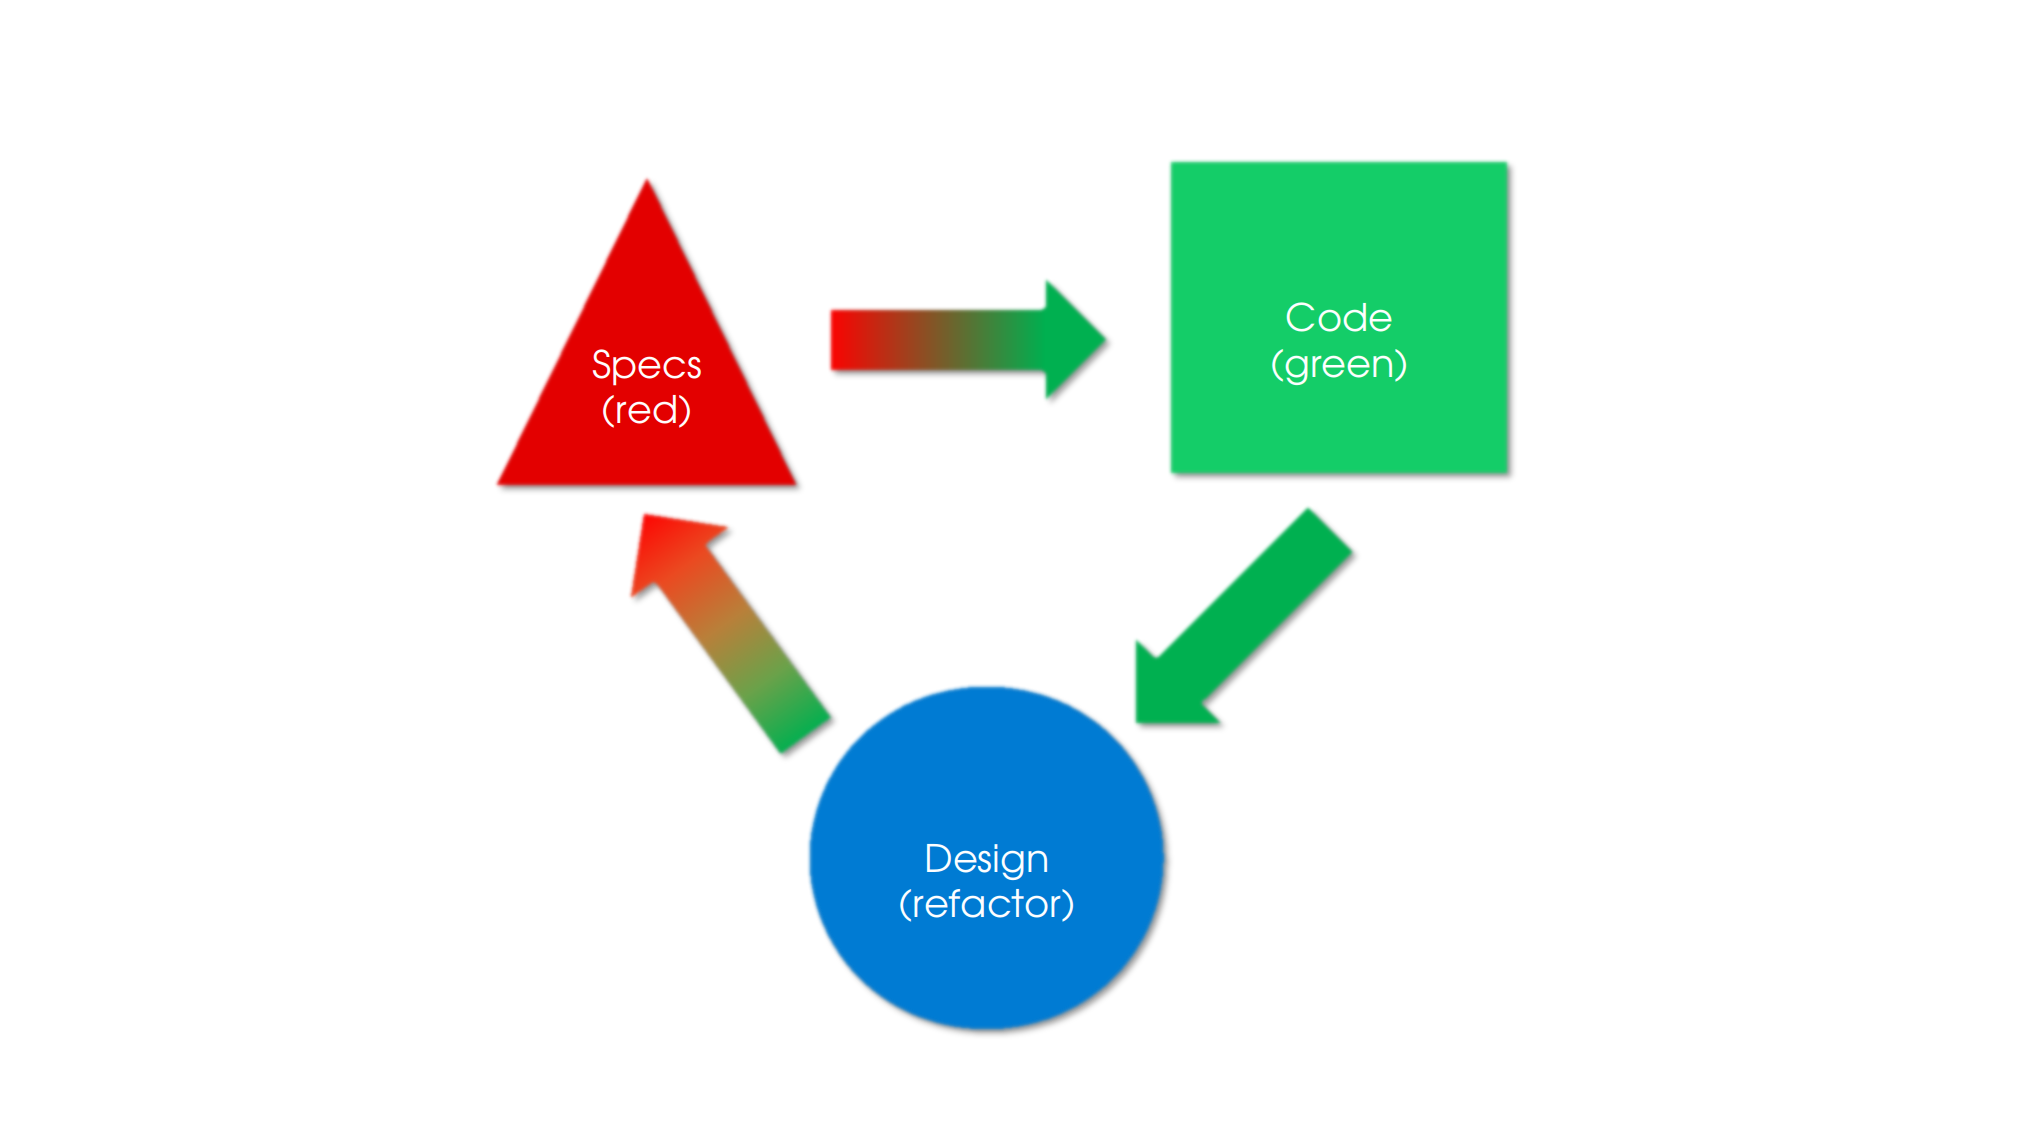
\includegraphics[width=\textwidth]{cycle}
    \note{
       On applique la même chose pour notre code.
       
       Red : On spécifie. On verifie que notre code ne fait pas déjà le job. On s'assure aussi que notre message d'erreur est explicite.

       Green : On fait passer le test le plus vite possible. On peut commiter au vert !

       Refactor : On améliore notre code sans en changer le comportement
    }
\end{frame}

\begin{frame}
    \begin{center}
        \Huge Démo
    \end{center}
\end{frame}
\end{document}
